\section{Information retrieval database}

Information retrieval databases adopt a search-engine-oriented architecture rather than a traditional database approach.
A prominent example is the ELK stack, which is structured into three key components:
\begin{itemize}
    \item \textit{Elasticsearch}: serves as the core of the stack and functions as a robust search and analytics engine. 
        It provides near real-time indexing, meaning documents become searchable shortly after being indexed. 
        Built on Apache Lucene, Elasticsearch enables full-text search capabilities, supports a distributed architecture for scalability and reliability, and uses a RESTful interface for easy integration with external systems.
    \item \textit{Logstash}: streaming ETL (Extract, Transform, Load) engine of the stack. 
        It facilitates centralized data collection, processing, and real-time enrichment. 
        Logstash is data agnostic, capable of handling various data formats, and supports a wide range of integrations and processors. 
    \item \textit{Kibana}: complements Elasticsearch by offering an open-source data visualization dashboard. 
        It allows users to create visual representations of the data indexed in Elasticsearch through an intuitive and straightforward interface. 
        Despite its simplicity, Kibana is highly customizable, enabling the creation of detailed and complex visualizations to suit specific needs.
\end{itemize}
\begin{figure}[H]
    \centering
    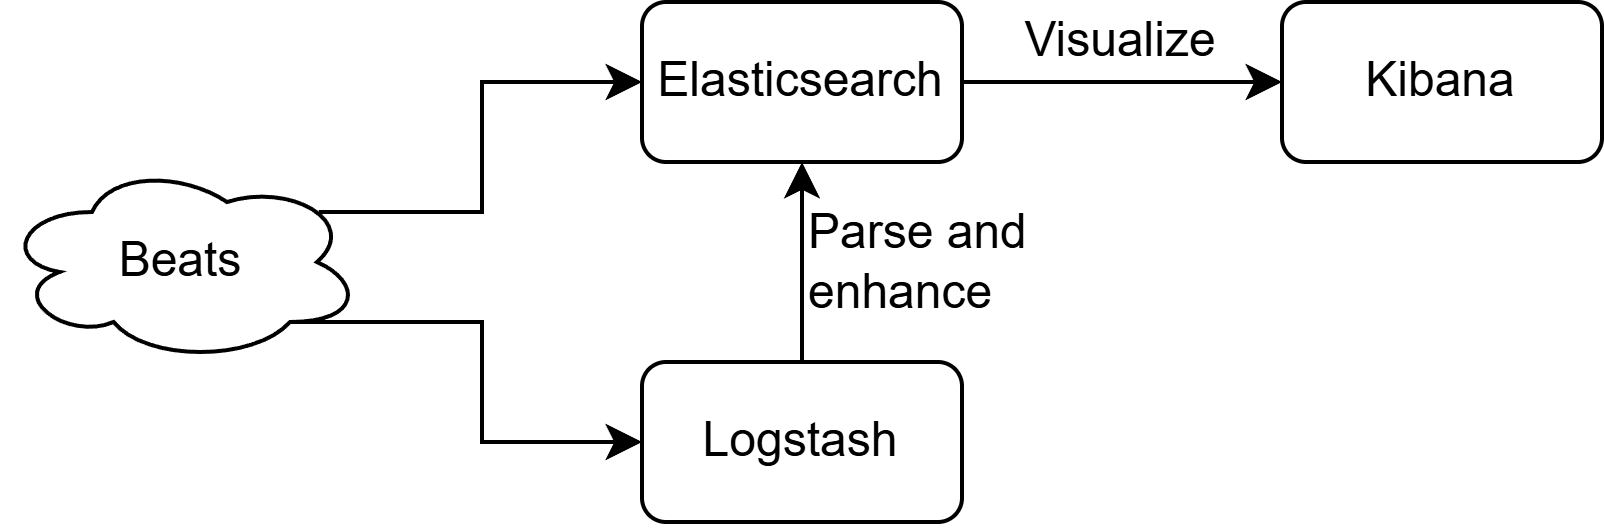
\includegraphics[width=0.75\linewidth]{images/elk.png}
    \caption{ELK stack}
\end{figure}

\subsection{Elasticsearch}
Elasticsearch introduces two features that are not typically found in traditional databases: 
\begin{itemize}
    \item \textit{Relevance}: relevance refers to how Elasticsearch handles query results. 
    In relational databases, a query retrieves data that exactly matches the specified conditions, returning a definitive answer. 
    In contrast, Elasticsearch prioritizes returning the best-matching elements rather than every possible match. 
    This is made possible through its use of an inverted index, which lists every unique word in all documents and maps each word to the documents in which it appears.

    Elasticsearch also organizes data using indexes, which define the structure of documents through mappings. 
    Each index is divided into shards, which help distribute operations across nodes to improve performance and resilience to faults. 
    Shards are further replicated into replicas, ensuring data redundancy by storing copies on different nodes for fault tolerance.
    \item \textit{Ranking}: unlike traditional databases, which often focus on returning all matches without prioritization, Elasticsearch determines the best and worst results for a query by calculating a relevance score. 
        This ranking system ensures that the most relevant elements are highlighted, making Elasticsearch particularly effective for search applications.

        Elasticsearch calculates the relevance of search results using Lucene's Practical Scoring Function, which incorporates TF-IDF (Term Frequency-Inverse Document Frequency). 
        TF-IDF is a statistical measure used to evaluate how important a term is within a document relative to a collection of documents. 
        This scoring method ensures that results are ranked according to their relevance to the query.
        We have the follwing elements: 
        \begin{itemize}
            \item \textit{Term frequency} (TF): the frequency of a term $i$ in a document $j$, normalized by the total number of terms in the document:
                \[\text{tf}_{i,j}=\dfrac{n_{i,j}}{\left\lvert d_j\right\rvert }\]
                Here, $n_{i,j}$ is the count of term $i$ in document $j$, and $\left\lvert d_j\right\rvert$ is the total number of terms in document $j$.
            \item \textit{Inverse document frequency} (IDF): this measures how unique or common a term is across the entire collection of documents. 
                Terms that appear in many documents are considered less significant. 
                The formula is:
                \[\text{idf}_i=\log\dfrac{\left\lvert D\right\rvert}{\left\lvert \left\{d\mid i\in d\right\}\right\rvert }\]
                Here, $\left\lvert D\right\rvert$ is the total number of documents, and $\left\lvert \left\{d\mid i\in d\right\}\right\rvert$ is the number of documents containing the term $i$.
        \end{itemize}
        The final TF-IDF score for a term $i$ in document $j$ is computed as the product of term frequency and inverse document frequency:
        \[(\text{tf-idf})_{i,j}=\text{tf}_{i,j}\times \text{idf}_i\]
\end{itemize}

\paragraph*{Mapping}
A mapping in Elasticsearch defines the structure and types of fields within an index. 
It determines: which fields are searchable, and support for full-text search, as well as time-based and geo-based queries.
However, mapping on an existing index cannot be changed once documents are stored. 
By default, Elasticsearch attempts to infer the structure of documents through dynamic mapping, which can be risky.




\subsubsection{Data model}
Elasticsearch stores data as JSON documents, making it easy to integrate with web applications. These documents are:
\begin{itemize}
    \item \textit{Distributed}: data can be accessed from any node within a cluster.
    \item \textit{Indexed}: newly stored documents are immediately indexed and made fully searchable.
\end{itemize}


\subsubsection{Query language}
Interaction with Elasticsearch is achieved by sending requests to REST endpoints, with actions determined by the following HTTP verbs:
\begin{itemize}
    \item \texttt{GET}: retrieve documents or index metadata.
    \item \texttt{POST/PUT}: create new documents or indices.
        \begin{itemize}
            \item \texttt{POST}: does not require an ID; Elasticsearch auto-generates one.
            \item \texttt{PUT}: requires an ID and is used to create or update a specific document.
        \end{itemize}
    \item \texttt{DELETE}: remove documents or indices.
\end{itemize}
Requests can be sent using: command-line tools, software like Postman, or developer tools in Kibana. 

\paragraph*{Indexing and mapping}
Indices and mappings are defined as follows:
\begin{lstlisting}[style=C]
PUT /index_name
\end{lstlisting} 
We can define a mapping in the following way: 
\begin{lstlisting}[style=C]
PUT /index_name/_mapping
\end{lstlisting} 
Common field types include:
\begin{itemize}
    \item \textit{Date}: for timestamps; formats can be specified.
    \item \textit{Keyword}: for structured data like emails, tags, and postcodes.
    \item \textit{Long}: for 64-bit integers.
    \item \textit{Text}: for full-text search, with customizable analyzers to preprocess data.
\end{itemize}


\paragraph*{Language analyzer}
Language analyzers preprocess text for search by: removing stopwords, and performing stemming to reduce words to their root forms.
\begin{lstlisting}[style=C]
POST /_analyze 
{
    text
}
\end{lstlisting} 
This returns a JSON structure optimized for the given input.

\paragraph*{Search}
To retrieve a document:
\begin{lstlisting}[style=C]
GET /index_name/type_name/id
\end{lstlisting} 
To perform a query:
\begin{lstlisting}[style=C]
GET /index_name/_search
{
    "query": {
        "match": {
            conditions
        }
    }
}
\end{lstlisting} 
To count matching documents:
\begin{lstlisting}[style=C]
GET /index_name/_count
{
    "query": {
        "match": {
            conditions
        }
    }
}
\end{lstlisting} 
Elasticsearch supports filters for exact matches, which are used for unanalyzed fields, do not calculate relevance (binary match), and are cacheable for performance.
Example of a query with filters:
\begin{lstlisting}[style=C]
GET /index_name/_search
{
    "query": {
        "bool": {
            "filter": {
                "term": { "field": "value" }
            }
        }
    }
}    
\end{lstlisting} 
Filters can be combined with queries to enhance efficiency and relevance scoring at query time. Elasticsearch also supports searching across multiple indices simultaneously.
The logical operators are must (AND), must not (NOT), and should (OR)

Elasticsearch provides a powerful aggregation framework to analyze data. 
Aggregations can be defined as follows:
\begin{lstlisting}[style=C]
GET /index_name/_search
{
    "query": {
        "size": 0,
        "aggs": {
            "aggregation_name": {
                "type": { "field": "field_name" }
            }
        }
    }
}
\end{lstlisting} 
Supported types of aggregations include:
\begin{itemize}
    \item \textit{Metrics}: summarize numeric data.
    \item \textit{Buckets}: group data into categories.
    \item \textit{Pipeline}: process results of other aggregations.
    \item \textit{Matrix}: perform advanced mathematical operations.
\end{itemize}
By combining queries, filters, and aggregations, Elasticsearch enables powerful data retrieval and analysis.

\subsection{Logstash}
Beats is a lightweight platform designed to serve as a data shipper, collecting and sending logs and metrics from hosts or containers to systems like Logstash or Elasticsearch. 
It includes several specialized modules, such as Filebeat for log file collection, Metricbeat for system and service metrics, Packetbeat for network data capture, and Heartbeat for monitoring service availability. 
These modules focus on data collection and shipping, while Logstash handles the more complex tasks of processing, structuring, normalizing, and enriching the data.
Logstash can also receive data from sources where Beats are not deployed, supporting protocols like TCP, UDP, HTTP, and pool-based inputs like JDBC.

\paragraph*{Processing}
Logstash uses filter plugins (or processors) for data wrangling. 
These filters help structure, normalize, and enrich incoming data, enabling users to build sophisticated data pipelines. 
These pipelines can be tailored to meet specific data processing needs, allowing for flexible and efficient management of diverse data types. 
After processing, Logstash can emit data to Elasticsearch or other data stores, using output plugins that support protocols such as TCP, UDP, and HTTP.

\paragraph*{Modules}
Logstash and Beats provide modules that facilitate automated processing for specific data types. 
These modules handle tasks like automated parsing and enrichment within Logstash, the creation of custom schemas in Elasticsearch, and the generation of default Kibana dashboards for data visualization.
These modules help streamline the process of transforming raw data into insightful visual representations, making it easier to integrate with Kibana for analysis.

\paragraph*{Data flow}
The flow of data in Logstash begins with the input, where data is ingested from various sources. 
It then passes through one or more filters, where it is structured, normalized, and enriched according to predefined rules. 
Finally, the processed data is emitted to the specified output, which could be Elasticsearch or another data store, or it could be sent to external systems via various protocols. 
This pipeline model ensures that data is efficiently managed, processed, and routed to the appropriate destination for further use or analysis.
\begin{figure}[H]
    \centering
    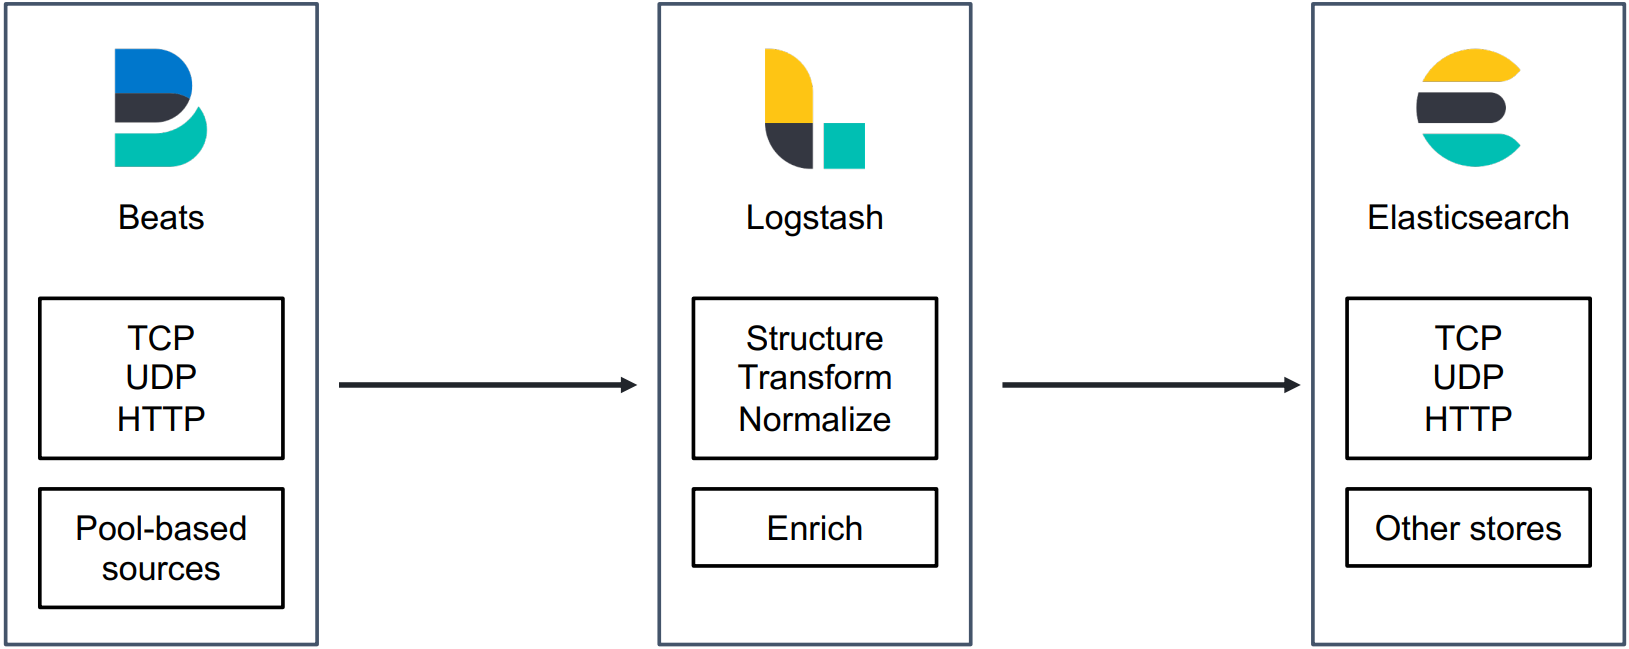
\includegraphics[width=0.75\linewidth]{images/ls.png}
    \caption{Logstash data flow}
\end{figure}

\subsubsection{Architecture}
In Logstash, the event is the primary unit of data, similar to a JSON document. 
These events flow through pipelines, which define the logical flow of data from ingestion to processing and output. 
A pipeline can handle multiple inputs simultaneously, managing the flow of data through a single queue, which can be configured to be either in-memory or persistent. 
This buffer ensures that data is processed in an organized manner, even under heavy load. 
Logstash employs workers to process the data, ensuring scalability by allowing multiple parallel processes to handle the incoming data efficiently.

Logstash instances can support multiple pipelines, each handling separate data flows independently. 
This makes it possible to configure different pipelines for distinct tasks within the same Logstash process.

To modify how data is represented, Logstash uses codecs to handle serialization and deserialization. 
Codecs are applied during data input or output, enabling flexibility in how data is processed as it moves through the system.

Logstash also employs an at least once message delivery strategy, which ensures that messages are generally delivered exactly once.
However, in the case of an unclean shutdown, duplicates may occur. 
To prevent data loss, Logstash utilizes a Dead Letter Queue for events that fail to be processed. 
This mechanism allows undeliverable events to be stored temporarily, freeing resources in the pipeline and ensuring that subsequent events are processed without delay.

\subsection{Kibana}
Kibana is an open-source data visualization tool designed specifically for Elasticsearch. 
It allows users to create interactive and dynamic visualizations based on the content indexed in an Elasticsearch cluster. 
While Kibana is intuitive and easy to use at first, it also offers a high degree of customization, enabling users to build complex and detailed representations of their data.
Regardless of the subscription level, Kibana provides robust capabilities to aggregate, organize, filter, and visualize data in various formats.
Kibana supports a wide array of visualizations, including charts, graphs, maps, and more. 
One of Kibana's most powerful features is the ability to create custom dashboards that integrate multiple data types and representations.